\documentclass[twoside]{book}

% Packages required by doxygen
\usepackage{fixltx2e}
\usepackage{calc}
\usepackage{doxygen}
\usepackage[export]{adjustbox} % also loads graphicx
\usepackage{graphicx}
\usepackage[utf8]{inputenc}
\usepackage{makeidx}
\usepackage{multicol}
\usepackage{multirow}
\PassOptionsToPackage{warn}{textcomp}
\usepackage{textcomp}
\usepackage[nointegrals]{wasysym}
\usepackage[table]{xcolor}

% Font selection
\usepackage[T1]{fontenc}
\usepackage[scaled=.90]{helvet}
\usepackage{courier}
\usepackage{amssymb}
\usepackage{sectsty}
\renewcommand{\familydefault}{\sfdefault}
\allsectionsfont{%
  \fontseries{bc}\selectfont%
  \color{darkgray}%
}
\renewcommand{\DoxyLabelFont}{%
  \fontseries{bc}\selectfont%
  \color{darkgray}%
}
\newcommand{\+}{\discretionary{\mbox{\scriptsize$\hookleftarrow$}}{}{}}

% Page & text layout
\usepackage{geometry}
\geometry{%
  a4paper,%
  top=2.5cm,%
  bottom=2.5cm,%
  left=2.5cm,%
  right=2.5cm%
}
\tolerance=750
\hfuzz=15pt
\hbadness=750
\setlength{\emergencystretch}{15pt}
\setlength{\parindent}{0cm}
\setlength{\parskip}{3ex plus 2ex minus 2ex}
\makeatletter
\renewcommand{\paragraph}{%
  \@startsection{paragraph}{4}{0ex}{-1.0ex}{1.0ex}{%
    \normalfont\normalsize\bfseries\SS@parafont%
  }%
}
\renewcommand{\subparagraph}{%
  \@startsection{subparagraph}{5}{0ex}{-1.0ex}{1.0ex}{%
    \normalfont\normalsize\bfseries\SS@subparafont%
  }%
}
\makeatother

% Headers & footers
\usepackage{fancyhdr}
\pagestyle{fancyplain}
\fancyhead[LE]{\fancyplain{}{\bfseries\thepage}}
\fancyhead[CE]{\fancyplain{}{}}
\fancyhead[RE]{\fancyplain{}{\bfseries\leftmark}}
\fancyhead[LO]{\fancyplain{}{\bfseries\rightmark}}
\fancyhead[CO]{\fancyplain{}{}}
\fancyhead[RO]{\fancyplain{}{\bfseries\thepage}}
\fancyfoot[LE]{\fancyplain{}{}}
\fancyfoot[CE]{\fancyplain{}{}}
\fancyfoot[RE]{\fancyplain{}{\bfseries\scriptsize Generated by Doxygen }}
\fancyfoot[LO]{\fancyplain{}{\bfseries\scriptsize Generated by Doxygen }}
\fancyfoot[CO]{\fancyplain{}{}}
\fancyfoot[RO]{\fancyplain{}{}}
\renewcommand{\footrulewidth}{0.4pt}
\renewcommand{\chaptermark}[1]{%
  \markboth{#1}{}%
}
\renewcommand{\sectionmark}[1]{%
  \markright{\thesection\ #1}%
}

% Indices & bibliography
\usepackage{natbib}
\usepackage[titles]{tocloft}
\setcounter{tocdepth}{3}
\setcounter{secnumdepth}{5}
\makeindex

% Hyperlinks (required, but should be loaded last)
\usepackage{ifpdf}
\ifpdf
  \usepackage[pdftex,pagebackref=true]{hyperref}
\else
  \usepackage[ps2pdf,pagebackref=true]{hyperref}
\fi
\hypersetup{%
  colorlinks=true,%
  linkcolor=blue,%
  citecolor=blue,%
  unicode%
}

% Custom commands
\newcommand{\clearemptydoublepage}{%
  \newpage{\pagestyle{empty}\cleardoublepage}%
}

\usepackage{caption}
\captionsetup{labelsep=space,justification=centering,font={bf},singlelinecheck=off,skip=4pt,position=top}

%===== C O N T E N T S =====

\begin{document}

% Titlepage & ToC
\hypersetup{pageanchor=false,
             bookmarksnumbered=true,
             pdfencoding=unicode
            }
\pagenumbering{roman}
\begin{titlepage}
\vspace*{7cm}
\begin{center}%
{\Large Rand\+Num\+Gen }\\
\vspace*{1cm}
{\large Generated by Doxygen 1.8.11}\\
\end{center}
\end{titlepage}
\clearemptydoublepage
\tableofcontents
\clearemptydoublepage
\pagenumbering{arabic}
\hypersetup{pageanchor=true}

%--- Begin generated contents ---
\chapter{File Index}
\section{File List}
Here is a list of all files with brief descriptions\+:\begin{DoxyCompactList}
\item\contentsline{section}{\hyperlink{arithmetic_mean_8c}{arithmetic\+Mean.\+c} }{\pageref{arithmetic_mean_8c}}{}
\item\contentsline{section}{\hyperlink{geometric_mean_8c}{geometric\+Mean.\+c} }{\pageref{geometric_mean_8c}}{}
\item\contentsline{section}{\hyperlink{harmonic_mean_8c}{harmonic\+Mean.\+c} }{\pageref{harmonic_mean_8c}}{}
\item\contentsline{section}{\hyperlink{means_8c}{means.\+c} }{\pageref{means_8c}}{}
\item\contentsline{section}{\hyperlink{means_8h}{means.\+h} }{\pageref{means_8h}}{}
\end{DoxyCompactList}

\chapter{File Documentation}
\hypertarget{average_8c}{}\section{average.\+c File Reference}
\label{average_8c}\index{average.\+c@{average.\+c}}
{\ttfamily \#include $<$math.\+h$>$}\\*
Include dependency graph for average.\+c\+:\nopagebreak
\begin{figure}[H]
\begin{center}
\leavevmode
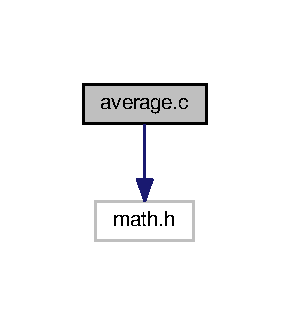
\includegraphics[width=139pt]{average_8c__incl}
\end{center}
\end{figure}
\subsection*{Functions}
\begin{DoxyCompactItemize}
\item 
float \hyperlink{average_8c_ac217ddafac7debd6e67f07590ef4e033}{average} (int sum, int len)
\end{DoxyCompactItemize}


\subsection{Function Documentation}
\index{average.\+c@{average.\+c}!average@{average}}
\index{average@{average}!average.\+c@{average.\+c}}
\subsubsection[{\texorpdfstring{average(int sum, int len)}{average(int sum, int len)}}]{\setlength{\rightskip}{0pt plus 5cm}float average (
\begin{DoxyParamCaption}
\item[{int}]{sum, }
\item[{int}]{len}
\end{DoxyParamCaption}
)}\hypertarget{average_8c_ac217ddafac7debd6e67f07590ef4e033}{}\label{average_8c_ac217ddafac7debd6e67f07590ef4e033}
Really, what do you think this does? It just divides something you idiot. It takes the sum of the generated numbers and divides by the amount of numbers generated. Idiot. 
\begin{DoxyParams}{Parameters}
{\em sum} & The sum of all the generated numbers. \\
\hline
{\em len} & The amount of all generated numbers. \\
\hline
\end{DoxyParams}

\hypertarget{lcg_8c}{}\section{lcg.\+c File Reference}
\label{lcg_8c}\index{lcg.\+c@{lcg.\+c}}
{\ttfamily \#include $<$math.\+h$>$}\\*
\subsection*{Functions}
\begin{DoxyCompactItemize}
\item 
int \hyperlink{lcg_8c_a961314425d451afd2d03cb36b0b74937}{lcg} (int seed, int mod)
\end{DoxyCompactItemize}


\subsection{Function Documentation}
\index{lcg.\+c@{lcg.\+c}!lcg@{lcg}}
\index{lcg@{lcg}!lcg.\+c@{lcg.\+c}}
\subsubsection[{\texorpdfstring{lcg(int seed, int mod)}{lcg(int seed, int mod)}}]{\setlength{\rightskip}{0pt plus 5cm}int lcg (
\begin{DoxyParamCaption}
\item[{int}]{seed, }
\item[{int}]{mod}
\end{DoxyParamCaption}
)}\hypertarget{lcg_8c_a961314425d451afd2d03cb36b0b74937}{}\label{lcg_8c_a961314425d451afd2d03cb36b0b74937}
The formula used to generate the psudeorandom numbers. 
\hypertarget{rand_num_gen_8c}{}\section{rand\+Num\+Gen.\+c File Reference}
\label{rand_num_gen_8c}\index{rand\+Num\+Gen.\+c@{rand\+Num\+Gen.\+c}}
{\ttfamily \#include $<$stdio.\+h$>$}\\*
{\ttfamily \#include $<$stdlib.\+h$>$}\\*
{\ttfamily \#include $<$math.\+h$>$}\\*
{\ttfamily \#include $<$time.\+h$>$}\\*
{\ttfamily \#include $<$unistd.\+h$>$}\\*
{\ttfamily \#include $<$sys/types.\+h$>$}\\*
{\ttfamily \#include $<$sys/stat.\+h$>$}\\*
{\ttfamily \#include $<$fcntl.\+h$>$}\\*
{\ttfamily \#include $<$string.\+h$>$}\\*
{\ttfamily \#include \char`\"{}rand\+Num\+Gen.\+h\char`\"{}}\\*
\subsection*{Macros}
\begin{DoxyCompactItemize}
\item 
\#define \hyperlink{rand_num_gen_8c_a78c99ffd76a7bb3c8c74db76207e9ab4}{\+\_\+\+X\+O\+P\+E\+N\+\_\+\+S\+O\+U\+R\+CE}~500
\end{DoxyCompactItemize}
\subsection*{Functions}
\begin{DoxyCompactItemize}
\item 
int \hyperlink{rand_num_gen_8c_a0ddf1224851353fc92bfbff6f499fa97}{main} (int argc, char $\ast$argv\mbox{[}$\,$\mbox{]})
\end{DoxyCompactItemize}


\subsection{Macro Definition Documentation}
\index{rand\+Num\+Gen.\+c@{rand\+Num\+Gen.\+c}!\+\_\+\+X\+O\+P\+E\+N\+\_\+\+S\+O\+U\+R\+CE@{\+\_\+\+X\+O\+P\+E\+N\+\_\+\+S\+O\+U\+R\+CE}}
\index{\+\_\+\+X\+O\+P\+E\+N\+\_\+\+S\+O\+U\+R\+CE@{\+\_\+\+X\+O\+P\+E\+N\+\_\+\+S\+O\+U\+R\+CE}!rand\+Num\+Gen.\+c@{rand\+Num\+Gen.\+c}}
\subsubsection[{\texorpdfstring{\+\_\+\+X\+O\+P\+E\+N\+\_\+\+S\+O\+U\+R\+CE}{_XOPEN_SOURCE}}]{\setlength{\rightskip}{0pt plus 5cm}\#define \+\_\+\+X\+O\+P\+E\+N\+\_\+\+S\+O\+U\+R\+CE~500}\hypertarget{rand_num_gen_8c_a78c99ffd76a7bb3c8c74db76207e9ab4}{}\label{rand_num_gen_8c_a78c99ffd76a7bb3c8c74db76207e9ab4}


\subsection{Function Documentation}
\index{rand\+Num\+Gen.\+c@{rand\+Num\+Gen.\+c}!main@{main}}
\index{main@{main}!rand\+Num\+Gen.\+c@{rand\+Num\+Gen.\+c}}
\subsubsection[{\texorpdfstring{main(int argc, char $\ast$argv[])}{main(int argc, char *argv[])}}]{\setlength{\rightskip}{0pt plus 5cm}int main (
\begin{DoxyParamCaption}
\item[{int}]{argc, }
\item[{char $\ast$}]{argv\mbox{[}$\,$\mbox{]}}
\end{DoxyParamCaption}
)}\hypertarget{rand_num_gen_8c_a0ddf1224851353fc92bfbff6f499fa97}{}\label{rand_num_gen_8c_a0ddf1224851353fc92bfbff6f499fa97}
Generates the random numbers and then checks to see if they appear random 1st argumnet is the amount of numbers generated

2nd argument is the seed of the random number generator

Takes the number generated by the formula. Puts it between 0 and 1. Then puts the number generated in the formula back agin to generate another number. Sum continues to calculate all the numbers generated.
\hypertarget{rand_num_gen_8h}{}\section{rand\+Num\+Gen.\+h File Reference}
\label{rand_num_gen_8h}\index{rand\+Num\+Gen.\+h@{rand\+Num\+Gen.\+h}}
\subsection*{Functions}
\begin{DoxyCompactItemize}
\item 
int \hyperlink{rand_num_gen_8h_ad6b35828af11c8f273bdec518bf11590}{lcg} (int sum, int mod)
\item 
float \hyperlink{rand_num_gen_8h_ac217ddafac7debd6e67f07590ef4e033}{average} (int sum, int len)
\end{DoxyCompactItemize}


\subsection{Function Documentation}
\index{rand\+Num\+Gen.\+h@{rand\+Num\+Gen.\+h}!average@{average}}
\index{average@{average}!rand\+Num\+Gen.\+h@{rand\+Num\+Gen.\+h}}
\subsubsection[{\texorpdfstring{average(int sum, int len)}{average(int sum, int len)}}]{\setlength{\rightskip}{0pt plus 5cm}float average (
\begin{DoxyParamCaption}
\item[{int}]{sum, }
\item[{int}]{len}
\end{DoxyParamCaption}
)}\hypertarget{rand_num_gen_8h_ac217ddafac7debd6e67f07590ef4e033}{}\label{rand_num_gen_8h_ac217ddafac7debd6e67f07590ef4e033}
Really, what do you think this does? It just divides something you idiot. It takes the sum of the generated numbers and divides by the amount of numbers generated. Idiot. \index{rand\+Num\+Gen.\+h@{rand\+Num\+Gen.\+h}!lcg@{lcg}}
\index{lcg@{lcg}!rand\+Num\+Gen.\+h@{rand\+Num\+Gen.\+h}}
\subsubsection[{\texorpdfstring{lcg(int sum, int mod)}{lcg(int sum, int mod)}}]{\setlength{\rightskip}{0pt plus 5cm}int lcg (
\begin{DoxyParamCaption}
\item[{int}]{seed, }
\item[{int}]{mod}
\end{DoxyParamCaption}
)}\hypertarget{rand_num_gen_8h_ad6b35828af11c8f273bdec518bf11590}{}\label{rand_num_gen_8h_ad6b35828af11c8f273bdec518bf11590}
The formula used to generate the psudeorandom numbers. 
%--- End generated contents ---

% Index
\backmatter
\newpage
\phantomsection
\clearemptydoublepage
\addcontentsline{toc}{chapter}{Index}
\printindex

\end{document}
